% \section{Sistemas Binarios}
\chapter{Sistemas Binarios}

La gran mayoría de sistemas estelares dentro de nuestra Galaxia no son aquellos
solitarios como nuestro propio sistema solar, si no que son compuestas de dos o
más estrellas ubicadas en corta aproximación de una a otra, a ordenes de
unidades astronómicas (AU por sus siglas en inglés). Estos sistemas multiples se
pueden clasificar con mayor precisión para aquellos compuestos de solo dos
estrellas, denominados como \textit{sistemas binarios}. Dentro de un sistema
binario la corta separación orbital entre ambas estrellas da como consecuencia a
fenómenos que surgen mediante la interacción entre las componentes, tanto como
la interacción gravitacional debido a sus masas, como a la física interesante
que ocurre en el caso de interacciones de material entre una estrella a otra. 

% TODO: incluir sección en cite?
Los sistemas binarios estelares ofrecen un laboratorio celeste de gran
importancia, ya que debido a la interacción a cortas escalas espaciales nos
brindan información acerca de las estrellas que sería imposible obtener de otra
manera. \citetbookchapter{phoebeScientificReference}{2.1} menciona varios
parámetros derivados de observaciones de estos sistemas, como las masas de cada
una de las componentes estelares por medio de su interacción gravitacional, la
calibración y estudio de la evolución estelar y su dependencia de la masa y
luminosidad de la estrella; dadas observaciones de sistemas desconectados, en el
cual ambas componentes son de la misma edad pero con diferentes propiedades que
influyen su camino evolutivo. La clasificación de estos sistemas se basa tanto
en propiedades observacionales\textemdash las cuales dependen tanto de las
propiedades geométricas del sistema como de nuestra capacidad de observación, en
cuanto a la capacidad de la instrumentación disponible\textemdash como en las
propiedades físicas del sistema, incluyendo la proximidad de las componentes
como sus propiedades lumínica.

\section{Geometría del Sistema - Modelo de Roche}

Es importante entender la forma geométrica de un sistema binario para llegar a
una descripción adecuada de ellos. Esto incluye los parámetros orbitales de las
estrellas tanto como la forma misma de ambas componentes, ya que en ciertos
casos tratar las estrellas como esferas rígidas da como resultado un modelo
incorrecto. A continuación se introduce las bases de las cuales se parte para
llegar a una representación de un sistema modelo, llegando a describir el
\textbf{modelo de Roche}.

Se define un sistema de coordenadas cartesiano tridimensional considerando un
marco de referencia no inercial, el cual está rotando con la misma velocidad que
las componentes del sistema binario orbitan una a otra. Esta es una
representación típica para el \textit{problema de tres cuerpos}, en el cual
tenemos a dos objetos masivos cuya influencia gravitacional se extiende al
espacio representado por el sistema de coordenadas. En la
\reffigure{figuraTresCuerpos} se puede ver este esquema, donde $m_1$ y $m_2$
representan ambas componentes estelares, posicionadas de tal manera que la
distancia entre las estrellas solo tenga una componente en una dirección
cartesiana.

\begin{figure}[!ht]
	\centering
	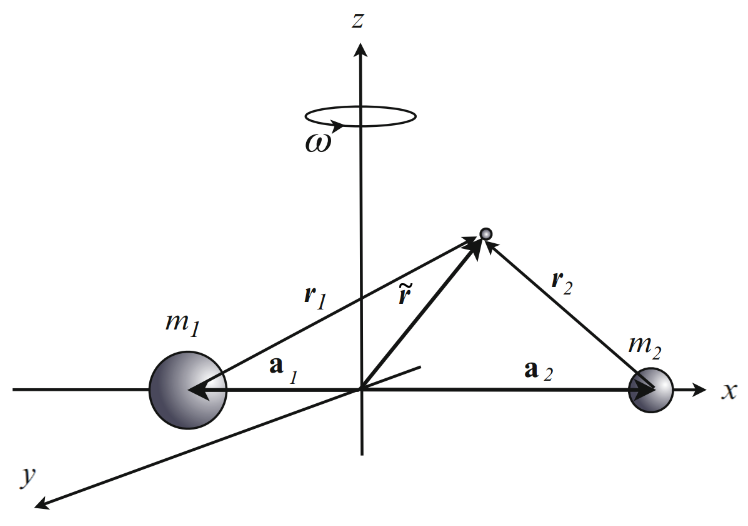
\includegraphics[scale=0.6]{Introduccion/Figures/Figura Tres Cuerpos_Intro Evolution Single Binary Stars.png}
	\caption{Configuración del problema de tres cuerpos dados dos objetos de
	alta masa $m_1$ y $m_2$ (las cuales representan cada componente estelar del
	sistema binario), y una partícula de masa despreciable de prueba ubicada a
	una distancia $r_1$ y $r_2$ de las estrellas respectivamente. El centro de
	masa del sistema está ubicado en el origen del sistema de coordenadas.
	Figura obtenida de
	\citetbookchapter{benacquista_introduction_to_evolution_single_binary_stars_2013}{13.1},
	modificada cambiando los ejes $y$ y $x$ para que $m_1$ y $m_2$ estén
	ubicadas en el eje $x$ para ser consistente con
	\citetbookchapter{phoebeScientificReference}{3.1}.}
	\label{figuraTresCuerpos}
\end{figure}

La \reffigure{figuraTresCuerpos} define el sistema de coordenadas rotando junto
al sistema binario. La velocidad angular de Kepler está dada por:

\begin{eqfloat}[!ht]
	\centering
	\begin{equation}
		\omega = \frac{2 \pi}{P_{orb}} = \sqrt{\frac{G (m_1 + m_2)}{a^3}}
	\end{equation}
	\blankcaption
	\label{ecuacionVelocidadAngular}
\end{eqfloat}

Donde $G = 6.673 \times 10^{-11} \ \mathrm{m}^3 \mathrm{kg}^{-1}
\mathrm{s}^{-2}$ es la constante de gravitación universal, $P_{orb}$ es el
periodo orbital de las estrellas (el cual es igual para ambas estrellas de
acuerdo a la segunda ley de Kepler), y $a = a_1 + a_2$ es el semieje mayor.
Usando la \refequation{ecuacionVelocidadAngular} podemos definir el Lagrangiano
para una partícula de prueba con masa $m$, el cual está a una distancia
$\mathbf{r}_1$ y $\mathbf{r}_2$ de $m_1$ y $m_2$ respectivamente:

\begin{eqfloat}[!ht]
	\centering
	\vspace{1em}
	\begin{equation}
		\Lagr = \eqnmark[MyDarkRed]{node1}{\frac{1}{2} m (\dot{x}^2 + \dot{y}^2 + \dot{z}^2)} +
				\eqnmark[MyDarkGreen]{node2}{\frac{1}{2} m \omega^2 \tilde{r}^2} +
				\eqnmark[MyDarkBlue]{node3}{\frac{G m_1 m}{r_1} + \frac{G m_2 m}{r_2}}
	\end{equation}
	\annotate[yshift=-0.2em]{below, left}{node1}{Energía cinética lineal}
	\annotate[yshift=0.75em]{above, left}{node2}{Energía cinética rotacional}
	\annotate[yshift=-0.75em]{below, left}{node3}{Potencial gravitacional}
	\blankcaption
	\vspace{0.4em}
	\label{ecuacionLagrangianoTresCuerpos}
\end{eqfloat}

Donde $\tilde{r}$ es la distancia al eje de rotación del marco de referencia,
$r_1 = \abs{\mathbf{r}_1} = \abs{\mathbf{r} - \mathbf{a}_1}$ y $r_2 =
\abs{\mathbf{r}_2} = \abs{\mathbf{r} - \mathbf{a}_2}$. Utilizando los últimos 3
términos de la \refequation{ecuacionLagrangianoTresCuerpos} podemos definir un
pseudo-potencial que determina el movimiento de la partícula de prueba, tanto
por la influencia gravitacional de las componentes como la fuerza centrifugal
dada por la rotación del marco de referencia. Esta ecuación se puede simplificar
al colocar el origen del sistema sobre la masa $m_1$ en vez de su centro de
masa, donde $x_{1} = 0$ es la posición de $m_1$ y $x_2 = \mathbf{a}_1 +
\mathbf{a}_2 = \mathbf{a}$ es la posición de la secundaria. Por lo tanto, la
nueva coordenada del centro de masa del sistema se da por:

\begin{eqfloat}[!ht]
	\centering
	\begin{equation}
		x_{\textrm{CoM}} = \frac{\sum_{i}{m_i x_i}}{\sum_{i}{m_i}} = \frac{qa}{1 + q}
	\end{equation}
	\blankcaption
	\label{ecuacionCentroDeMasa}
\end{eqfloat}

Donde introducimos un parámetro para la razón de masa $q = \frac{m_2}{m_1}$. En
varios trabajos las componentes de un sistema binario son identificados de tal
manera que $q \leq 1$; sin embargo, esta convención no suele ser conveniente al
momento de crear un modelo del sistema (por ejemplo,
\autocite{ding_fast_derivation_cbs_params_2022}), en donde se permite que $q > 1$
al asignar la componente primaria basado en parámetros orbitales. Esto se verá
más a profundidad al momento de describir el modelo computacional de un sistema
binario.
% TODO: incluir sección de PHOEBE una vez escrito

Este potencial efectivo $\psi$ se obtiene asumiendo una distribución de masa
esférica para ambas estrellas \citetbookchapter{phoebeScientificReference}{3.1}:

\begin{eqfloat}[!ht]
	\centering
	\begin{equation}
		\psi = -\frac{G m_1}{r_1} - \frac{G m_2}{r_2} - \frac{1}{2} \omega \tilde{r}^2
	\end{equation}
	\blankcaption
	\label{ecuacionPotencialEfectivo}
\end{eqfloat}

Usando el potencial $\psi$ es posible llegar a un potencial adimensional
$\Omega$ el cual determina la forma de ambas componentes. La geometría del
sistema se presta a un sistema de coordenadas esféricas, usando un ángulo polar
$\theta$ cuyo valor va desde $0$ en polo norte hasta $180^{\circ}$ en el polo
sur\textemdash paralelo al eje $z$ en la
\reffigure{figuraTresCuerpos}\textemdash y un ángulo azimutal $\phi$ cuyo valor
es $0$ en el eje $x$. Utilizamos las siguientes expresiones para convertir de
coordenadas cartesianas a coordenadas esféricas:

\begin{eqfloat}[!ht]
	\centering
	\begin{equation}
		\begin{split}
			& x = r \sin{\theta} \cos{\phi} = \lambda r \\
			& y = r \sin{\theta} \sin{\phi} = \mu r \\
			& z = r \cos{\theta} = \nu r
		\end{split}
	\end{equation}
	\blankcaption
	\label{ecuacionesCoordsEsfericasConversion}
\end{eqfloat}

En donde $r = \sqrt{x^2 + y^2 + z^2}$ es la distancia entre la partícula de
prueba ubicada en el punto $(x, y, z)$ al origen del sistema de coordenadas.
Partiendo del teorema de Pitágoras se puede llegar a una ecuación para calcular
la distancia $D$ entre dos puntos ubicados en $(x, y, z)$ y $(x', y', z')$ en un
sistema de coordenadas esférico:

\begin{eqfloat}[!ht]
	\centering
	\begin{equation}
		D = \sqrt{(x - x')^2 + (y - y')^2 + (z - z')^2}
	\end{equation}
\end{eqfloat}

La cual al expandir obtenemos:

\begin{eqfloat}[!ht]
	\centering
	\begin{equation}
		D = \sqrt{x^2 - 2xx' + x'^2 + y^2 - 2yy' + y'^2 + z^2 - 2zz' + z'^2}
		% D = \sqrt{\eqnmark[MyDarkBlue]{rNode1}{x^2} - 2xx' + x'^2 + \eqnmark[MyDarkBlue]{rNode2}{y^2} - 2yy' + y'^2 + \eqnmark[MyDarkBlue]{rNode3}{z^2} - 2zz' + z'^2}
	\end{equation}
\end{eqfloat}

Sustituyendo usando $d_1 = \sqrt{x^2 + y^2 + z^2}$ y $d_2 = \sqrt{x'^2 + y'^2 +
z'^2}$ como las distancias de ambos puntos al origen se obtiene:

\begin{eqfloat}[!ht]
	\centering
	\begin{equation}
		D = \sqrt{d_1^2 + d_2^2 - 2xx' - 2yy' -2zz'}
	\end{equation}
	\blankcaption
	\label{ecuacionDistanciaCartesiana}
\end{eqfloat}

Para obtener la distancia $D$ en coordenadas esféricas es necesario hacer la
conversión utilizando las \refequations{ecuacionesCoordsEsfericasConversion}, llegando a la expresión final:

\begin{eqfloat}[!ht]
	\centering
	\begin{equation}
		D = \sqrt{d_1^2 + d_2^2 - 2d_1d_2[(\sin{\theta} \sin{\theta'})(\cos{\phi - \phi'}) + \cos{\theta} \cos{\theta'}]}
	\end{equation}
	\blankcaption
	\label{ecuacionDistanciasEsferica}
\end{eqfloat}

Donde los puntos $(x, y, z)$ y $(x', y', z')$ corresponden a $(d_1, \theta,
\phi)$ y $(d_2, \theta', \phi')$ respectivamente. Se puede utilizar la
\refequation{ecuacionDistanciaCartesiana} y
\refequation{ecuacionDistanciasEsferica}\textemdash y haciendo uso de las
\refequations{ecuacionesCoordsEsfericasConversion}\textemdash para obtener las
distancias de la partícula de prueba $m$ a ambas componentes estelares del
sistema:

\begin{eqfloat}
	\centering
	\begin{equation}
		\begin{split}
			& r_1 = r \\
			& r_2 = \sqrt{r^2 - 2ax + a^2} = \sqrt{r^2 - 2ar\lambda + a^2} \\
			& \tilde{r} = \sqrt{(x - x_{\textrm{CoM}})^2 + y^2} = \sqrt{r^2(1 - \nu^2) - 2r\lambda x_{\textrm{CoM}} + x_{\textrm{CoM}}^2}
		\end{split}
	\end{equation}
	\blankcaption
	\label{ecuacionesDistancias}
\end{eqfloat}

Notando que el origen del sistema de coordenadas está ubicada en la posición de
la componente $m_1$. Por lo tanto, el potencial es definido con respecto a
$m_1$; para obtener el potencial con respecto a $m_2$ es necesario hacer una
transformación descrita en \citetbookchapter{phoebeScientificReference}{3.1}.
Sustituyendo las ecuaciones \refequations{ecuacionesDistancias} en la expresión
del potencial $\psi$ se obtiene el potencial efectivo en coordenadas esféricas:

\begin{eqfloat}[!ht]
	\centering
	\begin{equation}
		\psi(r, \lambda, \nu) = -\frac{Gm_1}{r} - \frac{Gm_2}{\sqrt{r^2 - 2ar\lambda + a^2}} - \frac{1}{2} \omega^2 (r^2(1-\nu^2) - 2r\lambda x_{\textrm{CoM}} + x_{\textrm{CoM}}^2)
	\end{equation}
	\blankcaption
	\label{ecuacionPotencialEfectivoEsferico}
\end{eqfloat}

Utilizando la tercera ley de Kepler de la forma $\omega^2 a^3 = G(m_1 + m_2)$
junto a la \refequation{ecuacionCentroDeMasa} y sustituyendo en la
\refequation{ecuacionPotencialEfectivoEsferico} se obtiene la forma final del
potencial efectivo, eliminando la dependencia explicita a la velocidad angular
del sistema y de la masa de la secundaria $m_2$
\citetbookchapter{phoebeScientificReference}{3.1}:

\begin{eqfloat}[!ht]
	\centering
	\begin{equation}
		\begin{split}
			\psi(r, \lambda, \nu) = -\frac{G m_1}{a} \left[ \frac{a}{r} + q \left(\frac{a}{\sqrt{r^2 - 2ar\lambda + a^2}} - \frac{r\lambda}{a} \right) \right.\\
			\left. + \frac{r^2}{2a^2}(1 + q)(1 - \nu^2) + \frac{q}{2(1 + q)} \right]
		\end{split}
	\end{equation}
	\blankcaption
	\label{ecuacionPotencialEfectivoFinal}
\end{eqfloat}

El potencial efectivo en la \refequation{ecuacionPotencialEfectivoFinal} se puede utilizar para definir un potencial adimensional, el cual define la forma de ambas componentes. Este potencial $\Omega$ se refiere al \textbf{potencial modificado de Kopal}, introducido en \citetbookchapter{kopal_close_binary_systems_1959}{III.1}. Este potencial se relaciona con $\psi$ por la siguiente ecuación:

\begin{eqfloat}[!ht]
	\centering
	\begin{equation}
		\Omega = -\frac{a \psi}{G m_1} - \frac{m_2^2}{2m_1(m_1 + m_2)}
	\end{equation}
\end{eqfloat}

El segundo término del RHS se puede simplificar multiplicando por $\frac{1/m_1^2}{1/m_1^2}$:

\begin{eqfloat}[!ht]
	\centering
	\begin{equation}
		\Omega = -\frac{a \psi}{G m_1} - \frac{q^2}{2(1 + q)}
	\end{equation}
	\blankcaption
	\label{ecuacionRochePotencialEfectivo}
\end{eqfloat}

Sustituyendo la \refequation{ecuacionPotencialEfectivoFinal} en
\refequation{ecuacionRochePotencialEfectivo} obtenemos obtenemos el potencial modificado
de Kopal:

\begin{eqfloat}[!ht]
	\centering
	\begin{equation}
		\Omega = \frac{1}{\varrho} + q\left(\frac{1}{\sqrt{\varrho^2 - 2\varrho \lambda + 1}} - \varrho \lambda \right) + \frac{1}{2} (1 + q)(1 - \nu^2)\varrho^2
	\end{equation}
	\blankcaption
	\label{ecuacionRoche}
\end{eqfloat}

Introduciendo la variable adimensional $\varrho = \frac{r}{a}$ usada en
\citetbookchapter{phoebeScientificReference}{3.1}. Usando la
\refequation{ecuacionRoche} podemos determinar la forma de ambas estrellas
asumiendo que la envoltura estelar (es decir, la capa superficial) coincide con
superficies de \textbf{equipotenciales de Roche}, donde el valor de $\Omega$ es
constante en toda la superficie
\citetbookchapter{kopal_close_binary_systems_1959}{3}. Este modelo de las
superficies estelares de un sistema binario comparte el nombre con el originador
de esta idea, el matemático francés \textit{Édouard Albert Roche} del siglo XIX.
Sin embargo, para que este modelo sea una buena aproximación del fenómeno
astrofísico debe de cumplir con las siguientes condiciones:

\begin{description}
	\item[Órbita circular sincrónica -] La formalización de los equipotenciales
	de Roche presentado en esta sección solo aplica para sistemas binarios cuya
	órbita es circular y sincrónica (los periodos de rotación de ambas estrellas
	son iguales al periodo orbital). 
	
	\item[Oscilaciones no-radiales despreciables -]  Las estrellas por
	imbalances locales padecen de una distorsión anisótropo, el cual causa que
	la superficie estelar se desvíe del modelo de Roche. Sin embargo, en la
	mayoría de las estrellas estas oscilaciones no-radiales ocurren en el orden
	de la escala de tiempo hidrostática, la cual, por ejemplo, es de ~15 minutos
	para una estrella tipo solar
	\citetbookchapter{kallrath_eclipsing_binary_modelling_2009}{3.1.5}. Mientras
	la escala de tiempo de estas distorsiones sea despreciable con respecto al
	periodo orbital la superficie estelar (su fotosfera) se puede parametrizar
	con el modelo de Roche.

	\item[Alta densidad de masa -] A pesar de que el material de una estrella
	esté distribuido por todo su volumen, el modelo de Roche simplifica la
	composición de una estrella a un punto infinitesimal el cual ejerce una
	fuerza gravitacional alrededor. Esta aproximación resulta en una superficie
	sin masa, cuya forma es dictada por el potencial de Roche. Esta aproximación
	permite derivar la expresión analítica en la \refequation{ecuacionRoche}, la
	cual se puede aplicar a fenómenos de alta \quotes{condensación central}
	\citetbookchapter{kopal_close_binary_systems_1959}{III}.
\end{description}

\subsection{Generalización a Órbitas Excéntricas y Asincrónicas}

% TODO: porqué no se puede modelar 
Una desventaja del modelo de Roche presentado en la \refequation{ecuacionRoche}
yace en sus suposiciones principales; como consecuencia de estas, el potencial
$\Omega$ definido hasta ahora solo puede ser aplicado a aquellos sistemas
binarios cuya órbita es circular y sincrónica. Esto excluye los sistemas con
órbitas excéntricas y/o asincrónicas, incluyendo sistemas binarios en contacto
cuyas propiedades no pueden ser adecuadamente modeladas en este paradigma
\citetbookchapter{kallrath_eclipsing_binary_modelling_2009}{3.1.5}.
\autocite{wilson_eccentric_1979} generaliza el modelo de Roche a este tipo de
órbitas, llegando a la siguiente expresión:

\begin{eqfloat}[!ht]
	\centering
	\begin{equation}
		\Omega = \frac{1}{\varrho} + q \left(\frac{1}{\sqrt{\delta^2 + \varrho^2 - 2\varrho \delta \lambda}} - \frac{\varrho \lambda}{\delta^2} \right) + \frac{F^2 \varrho^2 (1 + q)(1 - \nu^2)}{2}
	\end{equation}
	\blankcaption
	\label{ecuacionRocheExcentricaAsincronica}
\end{eqfloat}

Introduciendo dos términos: el \textit{parámetro de sincronicidad} $F =
\omega_{\mathrm{rot}} / \omega_{\mathrm{orb}}$ la razón de la velocidad angular rotacional de la
componente a su velocidad angular orbital, y la \textit{separación instantánea}
entre ambas componentes $\delta = D / a$ normalizada con respecto al semieje
mayor $a$ \citetbookchapter{phoebeScientificReference}{3.1}. El cambio principal
de este potencial modificado se refleja en la dependencia en la fase orbital del
campo potencial; debido a la excentricidad del sistema, las componentes no
mantienen una distancia constante una de otra, por lo cual el potencial de de
ser nuevamente calculado para cada fase. Al igual, este modelo considera
aquellos casos donde $F \neq 1$, ignorando los efectos de rotación diferencial
en las estrellas por simplicidad. Para el caso de una órbita sincrónica y
circular (es decir, $F = 1$ y $D = a$) la
\refequation{ecuacionRocheExcentricaAsincronica} se reduce a la
\refequation{ecuacionRoche}. Partiendo de esta ecuación se puede determinar la
forma de ambas estrellas.

\subsection{Superficies Equipotenciales}

La forma de una estrella en el modelo de Roche es determinada por una
\textbf{superficie equipotencial}, en la cual el valor del potencial $\Omega$ es
igual, identificado por un contorno. Una forma conveniente de definir la
superficie de un sistema es dando el valor de $\Omega$ en el polo norte de la
estrella primaria, en las coordenadas polares $(\theta = 0 \rightarrow \lambda = 0,\nu =
1)$; partiendo de este valor, incluyendo otros parámetros del sistema como la
razón de masa y el semieje mayor de la órbita, se define el contorno para el
valor del potencial del polo, denominado como $\Omega_{\mathrm{pol}}$. La
expresión para el potencial del polo se reduce a:

\begin{eqfloat}[!ht]
	\centering
	\begin{equation}
		\Omega_{\textrm{pol}} = \frac{1}{\varrho_{\textrm{pol}}} + \frac{q}{\sqrt{\delta^2 + \varrho_{\textrm{pol}}}}
	\end{equation}
	\blankcaption
	\label{ecuacionPotencialPoloRadio}
\end{eqfloat}

Donde $\Omega_{\textrm{pol}}$ es el valor del potencial modificado de Roche en
el polo de la estrella, y $\varrho_{\textrm{pol}}$ es el radio normalizado al
semieje mayor en el polo de la estrella. Usando esta expresión se puede
parametrizar la forma y tamaño de la estrella utilizando un solo valor para el
potencial; esto es gracias a la siguiente relación dada en
\citetbookchapter{phoebeScientificReference}{3.1}:

\begin{eqfloat}[!ht]
	\centering
	\begin{equation}
		\nabla p \parallel \rho \parallel \psi
	\end{equation}
\end{eqfloat}

% TODO: newpage para mantener formato de documento
\newpage

Esta nos dice que el gradiente de la densidad $\rho$, la presión $p$, y el
potencial efectivo $\psi$ son paralelo uno a otro, lo cual necesariamente
implica que una superficie constante del potencial coincide con las superficies
constantes de densidad y presión. Esta superficie equipotencial es resuelta
utilizando la \refequation{ecuacionPotencialPoloRadio} y
\refequation{ecuacionRocheExcentricaAsincronica}, dando el valor $\Omega =
\Omega_{\textrm{pol}}$ del sistema:

\begin{eqfloat}[!ht]
	\centering
	\begin{equation}
		\frac{1}{\varrho_{\textrm{pol}}} + \frac{q}{\sqrt{\delta^2 + \varrho_{\textrm{pol}}}} = \frac{1}{\varrho} + q \left(\frac{1}{\sqrt{\delta^2 + \varrho^2 - 2\varrho \delta \lambda}} - \frac{\varrho \lambda}{\delta^2} \right) + \frac{F^2 \varrho^2 (1 + q)(1 - \nu^2)}{2}
	\end{equation}
	\blankcaption
	\label{ecuacionRadioPolarEstelarEquivalencia}
\end{eqfloat}

Esta es resuelta de manera iterativa para cada valor de $\lambda$ y $\nu$ de la
malla de valores utilizada en el problema. El resultado es la forma de ambas
componentes del sistema binario, las cuales ya no son unas simples esferas o
incluso elipses, si no que toman una forma de gota que sigue el campo de
potencial establecido por medio de las fuerzas que rigen el sistema:

\begin{figure}[!ht]
	\centering
	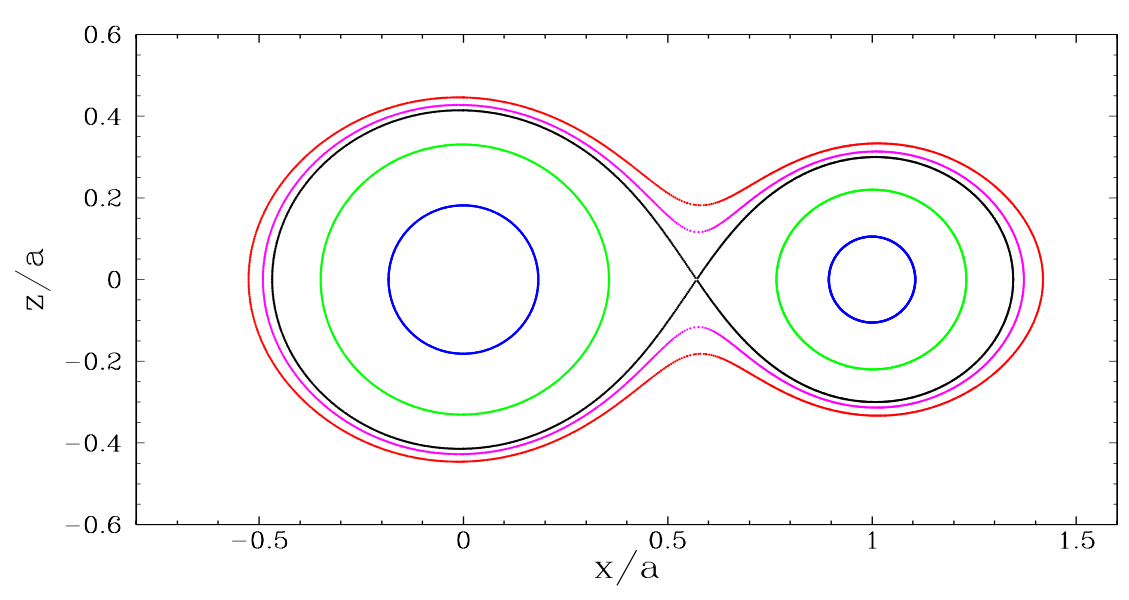
\includegraphics[scale=0.4]{Introduccion/Figures/Figura Forma Roche_PHOEBE Reference.png}
	\caption{Distintas formas de las componentes dependiendo del valor dado para $\Omega$. El potencial azul corresponde a $\Omega = 6.0$, verde a $\Omega = 3.5$, magenta a $\Omega = 2.8$, y rojo a $\Omega = 2.7$. La superficie negra corresponde a $\Omega = 2.87584$, el cual se le conoce como el \textbf{lóbulo de Roche crítico}. Figura obtenida de \citetbookchapter{phoebeScientificReference}{3.1}.}
	\label{figuraRocheFormaPhoebe}
\end{figure}

\section{Clasificación Morfológica}

Debido a que la estructura del potencial de Roche es una de las propiedades más
importantes para un sistema binario estelar, se acostumbran a clasificar en base
a la forma del potencial. Como se puede ver en la
\reffigure{figuraRocheFormaPhoebe}, diferentes valores para el potencial polar
$\Omega_{\mathrm{pol}}$ deforma ambas estrellas de maneras distintas, empezando
con componentes mayormente esféricas para altos valores de $\Omega$, hasta
llegar a sistemas en contacto en el caso de $\Omega < 2.87584$; la importancia
de este valor es explicada en esta sección.

\subsection{Sistemas Separados}

Los \textbf{sistemas separados} son aquellos cuya distancia orbital es
suficientemente grande para que las componentes estelares no hagan contacto
físico una con otra. Por lo tanto, estas componentes interactúan entre si
principalmente mediante sus campos gravitacionales, distorsionando la forma de
su compañera estelar. Las superficies estelares pueden ser mayormente esféricas
o elipsoidales dependiendo del campo de potencial, como se puede ver en la
\reffigure{figuraRocheFormaPhoebe} para los modelos que corresponden a $\Omega =
6.0$ y $\Omega = 3.5$. Estos sistemas son laboratorios importantes en el estudio
de las propiedades físicas de las estrellas, debido ńo solo a que permiten
calcular sus masas por medio de su interacción gravitacional, pero el hecho que
no tengan contacto físico permite estudiar las propiedades evolutivas de las
estrellas, ya que ambas componentes se desarrollan de manera independiente.

\subsection{Sistemas Semi-separados}

Un \textbf{sistema semi-separado} se distingue de otras morfologías debido a que
la separación orbital de las componentes estelares llega a ser del orden de
magnitud de unos cuantos radios solares. Esto causa que las superficies
equipotenciales de ambas estrellas se acerquen una a otra. En la
\reffigure{figuraRocheFormaPhoebe} se puede ver destacada la superficie de color
negro, en el cual el potencial de una componente está en contacto con su
compañera. Esta superficie se le conoce como el \textbf{lóbulo de Roche
crítico}, o simplemente como el \textbf{lóbulo de Roche}. El punto en el que
están en contacto es una región del espacio particular al problema de tres
cuerpos, que se le conoce como un \textit{punto de Lagrange}. Estas regiones del
espacio dentro del marco de referencia no-inercial marcan donde las fuerzas
ejercidas por el campo potencial de las componentes es igual a 0; una partícula
dentro de una de estas regiones no es sometida a ninguna aceleración. La
\reffigure{figuraLagrange} muestra las posiciones relativas de los puntos de
Lagrange.

\begin{figure}[!ht]
	\centering
	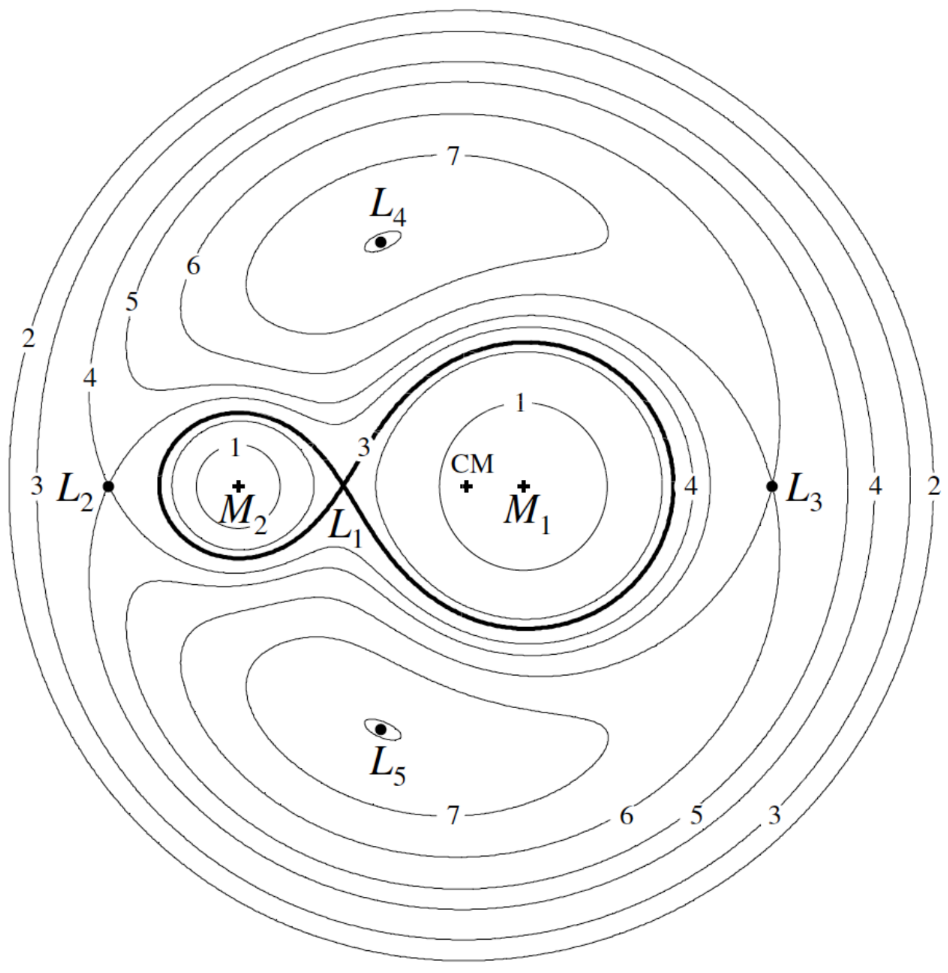
\includegraphics[scale=0.34]{Introduccion/Figures/Figura Lagrange_CVs Wide Field Surveys.png}
	\caption{El modelo de Roche para un sistema binario con una razón de masa $q
	= m_2 / m_1 = 0.25$. Se pueden apreciar los cinco puntos de
	Lagrange\textemdash \textit{L1}- \textit{L5}\textemdash que resultan del
	campo del potencial $\Omega$. Figura obtenida de
	\autocite{ibanez_cvs_wide_field_surveys_2021}.}
	\label{figuraLagrange}
\end{figure}

De interés particular es el punto \textit{L1}, el punto de contacto entre ambas
componentes. Una vez que una componente llene su lóbulo de Roche, el material
que previamente estaba ligado a su superficie será atraída gravitacionalmente a
la compañera estelar, iniciando un proceso de acreción de material. Las
\textit{variables cataclísmicas} son un ejemplo de este tipo de sistemas
binarios semi-separados, donde la componente secundaria enana roja llena su
lóbulo de Roche, transfiriendo material a la componente primaria enana blanca.

\subsection{Sistemas en Contacto}

Un sistema con un valor suficientemente pequeño de su potencial de Roche es un
\textbf{sistema binario en contacto}. A diferencia de un sistema semi-separado,
ambas componentes llenan su lóbulo de Roche en un sistema en contacto, haciendo
contacto en el punto de Lagrange \textit{L1}. Este caso de contacto (también
llamado un sistema en \textit{sobre-contacto} debido a que las estrellas no solo
están en contacto con su lóbulo de Roche, si no que su material se derrama fuera
del lóbulo crítico) da origen al fenómeno de una \textbf{envoltura común}: esta
es una superficie equipotencial que envuelve a ambas estrellas, en lugar de que
cada componente tenga su propia fotosfera independiente. La región de
conexión\textemdash conocida como el \quotes{cuello} del sistema por su nombre
en inglés\textemdash actúa como un puente entre las dos estrellas, sirviendo
como un medio de transporte de tanto material estelar como energía. Ejemplos de
superficies equipotenciales para estos sistemas se pueden ver en la
\reffigure{figuraRocheFormaPhoebe}, las cuales corresponden a $\Omega = 2.8$ y
$\Omega = 2.7$.

En el estudio de sistemas en contacto es importante introducir un nuevo
parámetro el cual describe la cantidad en que el sistema está en sobre-contacto.
El \textbf{factor de relleno}, por su nombre en inglés \textbf{fillout factor},
se define por medio de los valores del potencial en los puntos de Lagrange $L1
\rightarrow \Omega^{L1}_{\mathrm{crit}}$ y $L2 \rightarrow
\Omega^{L2}_{\mathrm{crit}}$:

\begin{eqfloat}
	\centering
	\begin{equation}
		\mathcal{F} = \frac{\Omega - \Omega^{L1}_{\textrm{crit}}}{\Omega^{L2}_{\textrm{crit}} - \Omega^{L1}_{\textrm{crit}}}
	\end{equation}
\end{eqfloat}

Esta ecuación describe la concentración espacial del material superficial de las
estrellas, definido unicamente con el potencial efectivo del sistema. El valor
del factor de relleno está restringido los siguientes valores: $\mathcal{F} < 0$
para sistemas separados, $\mathcal{F} = 0$ para el caso de semi-contacto, y $0 <
\mathcal{F} \leq 1$ para el caso de sobre-contacto. El factor de relleno resulta
ser una parametrización util al momento de modelar un sistema en contacto (por
ejemplo, utilizando el paquete de software \textit{PHOEBE}), debido a la
precisión computacional que sería necesaria para ajustar los radios individuales
de las estrellas. 

\section{Clasificaciones Observacionales}

Dependiendo del método de detección y las propiedades aparentes del sistema se
puede clasificar un sistema binario de estrellas. Estas clasificaciones son
independiente de sus propiedades físicas, como la clase espectral de cada
estrella o sus masas individuales. Al determinar su clasificación observacional
se puede delimitar las técnicas observacionales que son viables para recabar
datos del sistema; un sistema astrométrico sería indistinguible de uno
espectroscópico si uno intenta identificar las componentes individuales a simple
vista, o con un telescopio demasiado débil para el trabajo.

\begin{description}
	\item[Binarias visuales -] aquellos sistemas cuya separación orbital
	aparente es suficientemente grande para distinguir las dos estrellas
	individuales en la bóveda celeste. A pesar de que se puede trazar la órbita
	de la secundaria con varios años de observaciones, se requiere de cálculos
	adicionales para determinar la órbita exacta de las componentes. Esto se
	debe a la inclinación del sistema con respecto al eje de observación hacia
	la Tierra; solo es posible observar \quotes{una proyección del elipse
	orbital relativo en el plano del cielo,} aunque esto se puede superar usando
	el hecho de que la estrella primaria aparentemente inmóvil debe de estar
	presente \quotes{en un punto focal de la órbita relativa.}
	\citetbookchapter{fundamentalAstronomy}{10}

	\item[Binarias espectroscópicas -] presentan variaciones periódicas en sus
	espectros, en donde las líneas espectrales detectadas \quotes{oscilan
	periodicamente alrededor de la longitud de onda promedio}
	\citetbookchapter{astronomyPhysicalPerspective}{5}. Esto se observa debido
	al \textit{desplazamiento de Doppler}, lo cual causa que la frecuencia de un
	fotón se recorra hacia frecuencias más pequeñas (azules) o más grandes
	(rojas) dependiendo de su velocidad radial con respecto al observador, si se
	va acercando o alejando, respectivamente. Estas también pueden ser identificadas
	al observar dos distintos grupos de líneas espectrales, el cual es resultado
	de la contribución de ambas estrellas.

	\item[Binarias astrométricas -] al igual que las espectroscópicas, las
	binarias astrométricas solo muestran una componente visible al ser
	observada, al contrario de las binarias visibles. Sin embargo, una binaria
	astrométrica difiera de las otras dos categorías definidas en cuestión de su
	movimiento observado en la bóveda celeste. Estas muestran un movimiento
	errático y no-lineal, algo que no se esperaría ver en una estrella solitaria
	dado su inercia según la primera ley de Newton. Estas perturbaciones son
	causadas por una estrella secundaria no aparente al observar el sistema. 
\end{description}

\section{Binarias Eclipsantes}

Una de las propiedades más útiles de identificar de un sistema binario es
la \textit{inclinación} de su órbita con respecto a la línea de visión
del sitio de observación (ya sea la Tierra en caso de un observatorio
terrestre o un punto lejano dentro del sistema solar para un telescopio
espacial). En dado caso que un sistema tenga una inclinación suficientemente
alta se pueden observar eclipses dentro del sistema, en lo que una componente
obscurece a su compañera de nuestra línea de visión, otorgando el nombre de 
\textbf{binaria eclipsante} a los sistemas que muestran este fenómeno. 
Aparte de su clasificación morfológica física, los sistemas binarios eclipsantes
se pueden distinguir en 3 diferentes tipos de sistemas binarios cercanos,
basados en la forma de su curva de luz.

\subsection{EA - Algol}

Las curvas de luz de tipo \textit{EA} son atribuidas generalmente a sistemas
binarios separados, donde ambas componentes estelares pueden mantener su forma
esférica sin perturbaciones a escalas apreciables. Gracias a esta separación de
las estrellas es posible definir claramente el comienzo y fin de ambos eclipses;
fuera de los eclipses, la curva de luz se mantiene relativamente constante,
mostrando variabilidad despreciable en casos de variabilidad elipsoidal (en el
caso que las componentes no sean esferas perfectas debido a una leve distorsión
por el potencial gravitacional) o en caso del calentamiento superficial de una
componente por la radiación incidente de su compañera
\autocite{samus_gcvs_variable_types_2016}. Existen sistemas con un rango amplio
de periodos orbitales, desde 4 horas hasta más de 25 años. Una curva de luz
típica de un sistema \textit{EA} se puede apreciar en la
\reffigure{figuraEACurvaLuz}.

\begin{figure}[!ht]
	\centering
	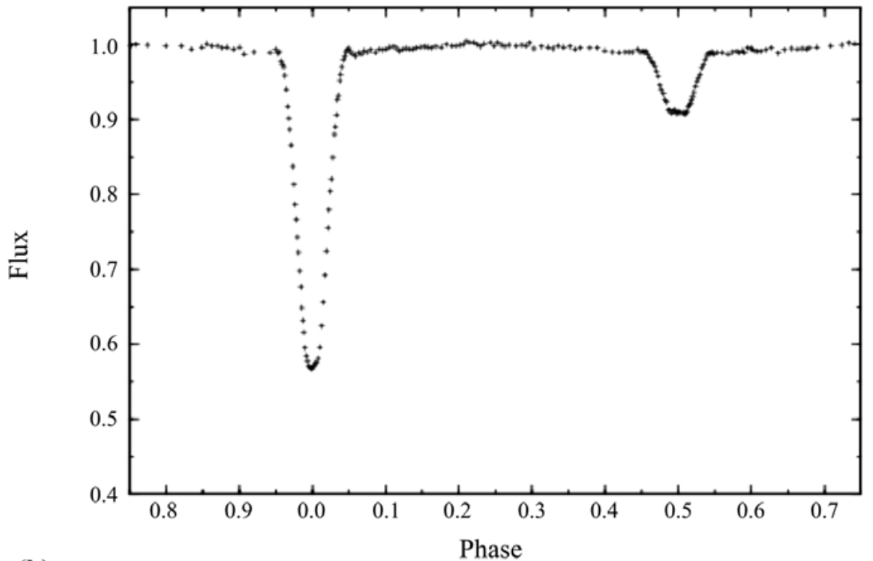
\includegraphics[scale=0.6]{Introduccion/Figures/Figura EA Curva_Modelling of WUMa Stars.png}
	\caption{Curva de luz emblemática de un sistema eclipsante
	\textit{EA}. Obtenida de
	\autocite{skelton_modelling_wuma_variable_stars_2009}.}
	\label{figuraEACurvaLuz}
\end{figure}

\subsection{EB - \textbeta \ Lyrae}

En el caso de un sistema eclipsante semi-separado, la curva de luz observada se
le clasifica como tipo \textit{EB}, o de tipo \textbeta \space Lyrae. En un sistema
semi-separado una de las estrellas llena su lóbulo crítico de Roche, haciendo
contacto con la superficie de su compañera. Esta distorsión es responsable de su
forma elipsoidal en vez de esférica. El flujo que un observador recibe de una
estrella es proporcional al área superficial visible en la línea de visión; en
una estrella esférica, esta área es constante en el tiempo, pero en el caso de
una estrella elipsoidal la cantidad de área observada depende de la fase orbital
actual. Esto resulta en eclipses sin un comienzo y fin claramente delimitados.
En la mayoría de los casos el periodo orbital de este tipo de sistemas es mayor
de 1 día \autocite{samus_gcvs_variable_types_2016}. 

\begin{figure}[!ht]
	\centering
	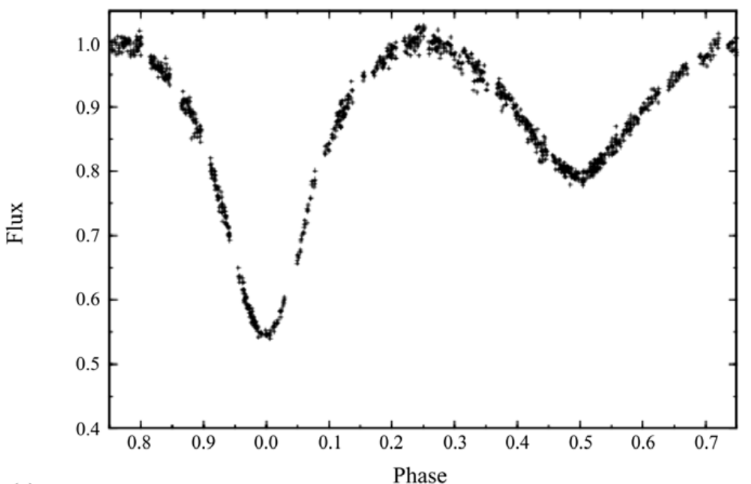
\includegraphics[scale=0.63]{Introduccion/Figures/Figura EB Curva_Modelling of WUMa Stars.png}
	\caption{Curva de luz emblemática de un sistema eclipsante
	\textit{EB}. Obtenida de
	\autocite{skelton_modelling_wuma_variable_stars_2009}.}
	\label{figuraEBCurvaLuz}
\end{figure}

\subsection{EW - W UMa}

Sistemas en sobre-contacto, en donde ambas componentes llenan su lóbulo de
Roche, producen curvas de luz que muestran variabilidad continua a lo largo de
su órbita, parecido a los sistemas \textit{EB}. Sin embargo, a diferencia de los
sistemas semi-separados, ambas componentes de sistemas tipo \textit{EW} están
altamente acopladas una a otra, la diferencia de temperaturas siendo del orden
de cientos de Kelvin\textemdash lo cual es evidente por la profundidad de ambos
eclipses\textemdash de tipo espectral A-K
\autocite{skelton_modelling_wuma_variable_stars_2009}. El periodo orbital es
menor de 1 día, del orden de unas cuantas horas, debido a su corta aproximación
física. La envoltura común que comparten las estrellas es de una forma
irregular; esta consiste de las superficies elipsoidales de las estrellas y del
\quotes{cuello}, la región que llena el espacio alrededor del punto de Lagrange
L1. Debido a esta geometría, cada fase orbital muestra una cantidad distinta de
la superficie del sistema, causando la variabilidad continua en la curva de luz,
sin una clara delimitación para ninguno de los eclipses. La
\reffigure{figuraEWCurvaLuz} muestra una curva de luz típica de un sistema
\textit{EW}. 

Una característica única de los sistemas \textit{EW} es la diferencia en los
máximos de la curva de luz. En ciertos casos puede ocurrir que un máximo del
flujo sea mayor que el máximo medido de el eclipse contrario, a pesar de estar
viendo una cantidad similar de superficie estelar. Este fenómeno observacional
es denominado el \textit{efecto O'Connell}. A pesar de que aún no es muy bien
entendido la causa de este efecto, una de las interpretaciones más populares en
la literatura es la presencia de manchas estelares
[\autocite{ding_fast_derivation_cbs_params_2022}
\autocite{michel_photometric_study_contact_binary_2023}
\autocite{michel_rotse1_new_wuma_eclipsing_binary_2016}], las cuales al ser más
frías que el resto de la superficie llega a manifestar como una menor cantidad
de radiación emitida por el sistema en ciertas fases. Esto se atribuye a la
actividad magnética de la estrella, y se utiliza principalmente al momento de
ajustar un modelo computacional a la curva de luz observada.

\begin{figure}[!ht]
	\centering
	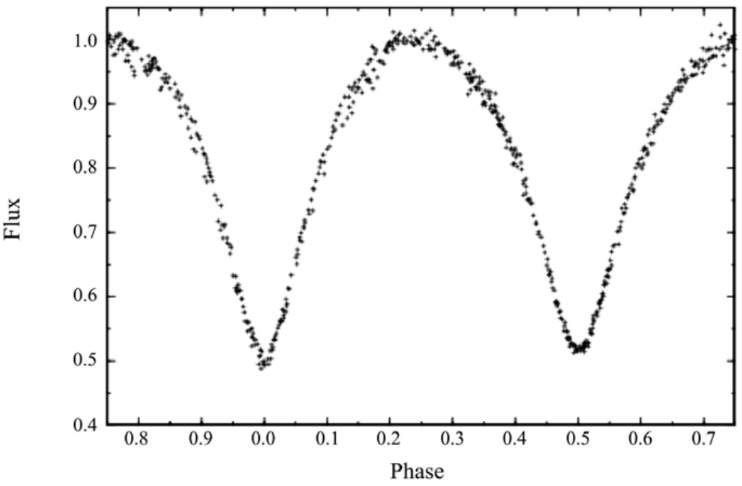
\includegraphics[scale=0.63]{Introduccion/Figures/Figura EW Curva_Modelling of WUMa Stars.png}
	\caption{Curva de luz emblemática de un sistema eclipsante
	\textit{EW}. Obtenida de
	\autocite{skelton_modelling_wuma_variable_stars_2009}.}
	\label{figuraEWCurvaLuz}
\end{figure}